\section{Capacitatea disponibilă}

\begin{frame}{Capacitatea disponibilă}
  \begin{itemize}
    \item Throughput mare
    \item Mulți factori
    \begin{itemize}
      \item Calitatea canalului
      \item Distanța dintre client și AP
      \item Traficul efectuat de alți clienți
      \item Algoritmii de autorate ai clientului
    \end{itemize}
    \item Timpul liber pe canal și rata de transmisie estimată
  \end{itemize}
\end{frame}

\begin{frame}{Timpul liber pe canal}
  \begin {columns}
  \begin {column}{0.5\linewidth}
  \begin{itemize}
    \item Downlink, uplink, interferență
    \item Metodă asemănătoare ProbeGap
    \begin{itemize}
      \item Timpul de când se pune un pachet în coadă până când este transmis
      \item Se determină timpul de transmisie când canalul este liber
      \item Canalul este ocupat când transmisia durează mai mult
    \end{itemize}
  \end{itemize}
  \end{column}
  \begin {column}{0.5\linewidth}
      \begin{figure}
        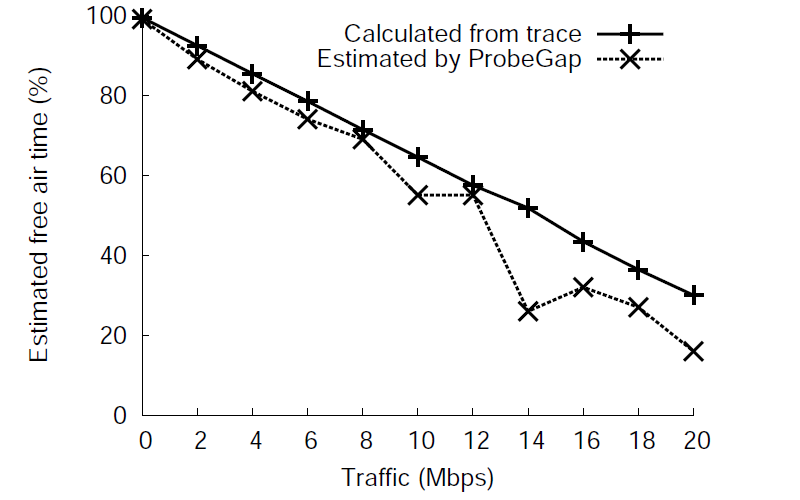
\includegraphics[scale=0.20]{img/fig4.png}
      \end{figure}
  \end{column}
  \end{columns}
\end{frame}
  
\begin{frame}{Rata de transmisie}
  \begin{itemize}
    \item ProbeRequest
    \item RSSI - tabelă de mapare
    \item Pe distanțe scurte este precis
    \item Multe AP-uri, probabil va fi select unul apropiat
  \end{itemize}
\end{frame}
